

\gaokaoheader{2020}{全国\lmd{1}卷}



\gaokaoxz




\begin{enumerate}
\item
行驶中的汽车如果发生剧烈碰撞,车内的安全气囊会被弹出并瞬间充满气体。若碰
撞后汽车的速度在很短时间内减小为零,关于安全气囊在此过程中的作用,下列说
法正确的是 \xzanswer{D} 


\fourchoices
{增加了司机单位面积的受力大小}
{减少了碰撞前后司机动量的变化量}
{将司机的动能全部转换成汽车的动能}
{延长了司机的受力时间并增大了司机的受力面积}


%题目类型:选择
%题目区域:动量:冲量
%题目难度:9
%思想方法:
%题目特征:材料分析
%题目备注:



\item 
火星的质量约为地球质量的$ 1/10 $,半径约为地球半径的$ 1/2 $,则同一物体在火星表
面与在地球表面受到的引力的比值约为 \xzanswer{B} 

\fourchoices
{0.2}
{0.4}
{2.0}
{2.5}

%题目类型:选择
%题目区域:万有引力
%题目难度:8
%思想方法:	
%题目特征:
%题目备注:

\item 
如图,一同学表演荡秋千,已知秋千的两根绳长均为$ 10 \ m $,该同学
和秋千踏板的总质量约为$ 50 \ kg $,绳的质量忽略不计,当该同学荡到
秋千支架的正下方时,速度大小为$ 8 \ m/s $,此时每根绳子平均承受的
拉力约为 \xzanswer{B} 
% TODO: \usepackage{graphicx} required
\begin{figure}[h!]
\centering
%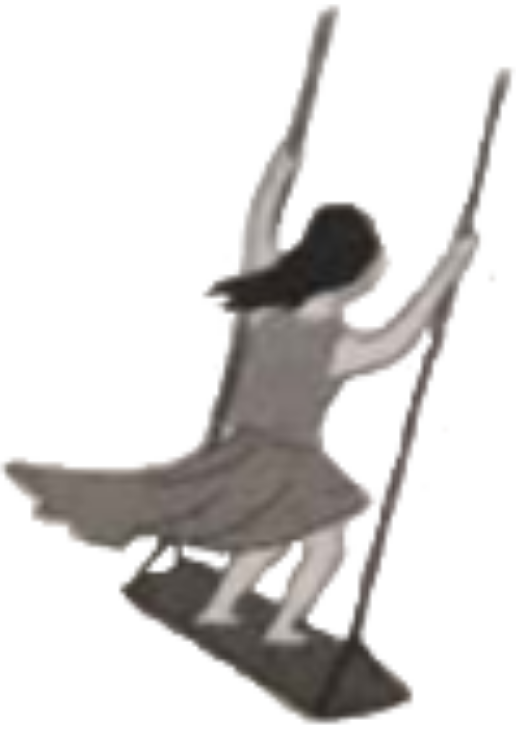
\includegraphics[width=0.12\linewidth]{picture/screenshot034}
 \includesvg[width=0.16\linewidth]{picture/svg/GZ-3-tiyou-0608} 
\end{figure}



\fourchoices
{$ 200 \ N $}
{$ 400 \ N $}
{$ 600 \ N $}
{$ 800 \ N $}

%题目类型:选择
%题目区域:曲线运动:圆周
%题目难度:7
%思想方法:
%题目特征:材料分析
%题目备注:荡秋千的过程,轨迹为一圆。


\item 
图 \subref{2020-4-a} 所示的电路中,$ K $与$ L $间接一
智能电源,用以控制电容器$ C $两端的
电压$ U_{c} $,如果$ U_{c} $随时间$ t $的变化如图
\subref{2020-4-b} 所示,则下列描述电阻$ R $两端电
压$ U_{R} $随时间$ t $变化的图像中,正确的是 \xzanswer{A} 
\begin{figure}[h!]
\centering
\begin{subfigure}{0.4\linewidth}
\centering
\includesvg[width=0.5\linewidth]{picture/svg/GZ-3-tiyou-0615} 
\caption{}\label{2020-4-a}
\end{subfigure}
\hfil
\begin{subfigure}{0.4\linewidth}
\centering
\includesvg[width=0.7\linewidth]{picture/svg/GZ-3-tiyou-0616} 
\caption{}\label{2020-4-b}
\end{subfigure}
%\includesvg[width=0.83\linewidth]{picture/svg/GZ-3-tiyou-0592}
 %\includesvg[width=0.53\linewidth]{picture/svg/GZ-3-tiyou-0607}\\ 
 %\vspace{0.5em}
 %\includesvg[width=0.63\linewidth]{picture/svg/GZ-3-tiyou-0606} 
\end{figure}



\pfourchoices
{\includesvg[width=4.3cm]{picture/svg/GZ-3-tiyou-0611}}
{\includesvg[width=4.3cm]{picture/svg/GZ-3-tiyou-0612}}
{\includesvg[width=4.3cm]{picture/svg/GZ-3-tiyou-0613}}
{\includesvg[width=4.3cm]{picture/svg/GZ-3-tiyou-0614}}



%题目类型:选择
%题目区域:电路
%题目难度:6
%思想方法:
%题目特征:图像选择
%题目备注:利用排除法即可快速选出。


\item 
一匀强磁场的磁感应强度大小为$ B $,方向垂直于纸面向外,其边界如图中虚线所示,
$ \overarc{ab} $为半圆,$ ac $、$ bd $与直径$ ab $共线,$ ac $间的距离等于半圆的半径。一束质量为$ m $、
电荷量为$ q(q>0) $的粒子,在纸面内从$ c $点垂直于$ ac $射
入磁场,这些粒子具有各种速率,不计粒子之间的相互作用。在磁场中运动时间最长的粒子,其运动时间为 \xzanswer{C} 
\begin{figure}[h!]
\centering
\includesvg[width=0.3\linewidth]{picture/svg/GZ-3-tiyou-0596}
\end{figure}




\fourchoices
{$\frac{7 \pi m}{6 q B}$}
{$\frac{5 \pi m}{4 q B}$}
{$\frac{4 \pi m}{3 q B}$}
{$\frac{3 \pi n}{2 q B}$}


%题目类型:选择
%题目区域:磁场
%题目难度:4
%思想方法:
%题目特征:
%题目备注:过$ c $点作$ \overarc{ab} $的切线,交点处即为运动时间最长的点。

\item 
下列核反应方程中, \ce{X_1} 、 \ce{X_2} 、 \ce{X_3} 、 \ce{X_4} ,代表$ \alpha $粒子的有 \xzanswer{BD} 

\fourchoices
{ \ce{_{1}^{2}H + ^{2}_{1}H \rightarrow ^{1}_{0} n + X_{1} }}
{\ce{^{2}_{1}H + ^{3}_{1}H \rightarrow ^{1}_{0}n + X_{2} }}
{ \ce{^{235}_{92}H + ^{1}_{0}n \rightarrow ^{144}_{56}Ba + ^{89}_{36}Kr + 3X_{3} }}
{ \ce{ ^{1}_{0} n + \ce{^{6}_{3}Li} \rightarrow ^{3}_{1}H + X_{4} }}

%题目类型:选择
%题目区域:原子物理
%题目难度:8
%思想方法:
%题目特征:


\item 
一物块在高$ 3.0 \ m $、长$ 5.0 \ m $的斜面顶端从静止开始沿斜
面下滑,其重力势能和动能随下滑距离$ s $的变化如图中
直线 \lmd{1} 、 \lmd{2} 所示,重力加速度取$ 10 \ m/s^{2} $,则 \xzanswer{AB} 
\begin{figure}[h!]
\centering
\includesvg[width=0.3\linewidth]{picture/svg/GZ-3-tiyou-0594}
\end{figure}



\fourchoices
{物块下滑过程中机械能不守恒}
{物块与斜面间的动摩擦因数为$ 0.5 $}
{物块下滑时加速度的大小为$ 6.0 \ m/s^{2} $}
{当物块下滑$ 2.0 \ m $时机械能损失了$ 12 \ J $}


%题目类型:选择
%题目区域:能量守恒:动能定理
%题目难度:5
%思想方法:
%题目特征:图像分析
%题目备注:利用好斜率与截距,即可快速完成。


\item 
如图,$ U $形光滑金属框$ abcd $置于水平绝缘平台上,$ ab $和$ dc $边平行,和$ bc $边垂直。
$ ab $、$ dc $足够长,整个金属框电阻可忽略,一根具有一定电阻的导体棒$ MN $置于金属
框上,用水平恒力$ F $向右拉动金属框,运动过程中,装置始终处于竖直向下的匀强
磁场中,$ MN $与金属框保持良好接触,且与$ bc $边保持平行。经过一段时间后 \xzanswer{BC} 

\begin{figure}[h!]
\centering
\includesvg[width=0.33\linewidth]{picture/svg/GZ-3-tiyou-0597}
\end{figure}


\fourchoices
{金属框的速度大小趋于恒定值}
{金属框的加速度大小趋于恒定值}
{导体棒所受安培力的大小趋于恒定值}
{导体棒到金属框$ bc $边的距离趋于恒定值}

%题目类型:选择
%题目区域:磁场
%题目难度:3
%思想方法:极限:假设:隔离
%题目特征:
%题目备注:最终状态是速度之差恒定,对应两种情况:一是二者匀速,二是二者加速度相等。




\gaokaosy

\item 
某同学用伏安法测量一阻值为几十欧姆的电阻$ R_{x}$,所用电压
表的内阻为$ 1 \ K\Omega $,电流表内阻为$ 0.5 \ \Omega $,该同学采用两种测量方案,
一种是将电压表跨接在图 \subref{2020:全国1:9a} 所示电路的$ O $、$ P $两点之间,另一
种是跨接在$ O $、$ Q $两点之间,测量得到如图 \subref{2020:全国1:9b} 所示的两条$ U-I $图线,其中$ U $与$ I $分
别为电压表和电流表的示数。
\begin{figure}[!htp]
\centering
%\includesvg[width=0.3\linewidth]{picture/svg/GZ-3-tiyou-0598}
% \includesvg[width=0.3\linewidth]{picture/svg/GZ-3-tiyou-0609} 
\begin{subfigure}{0.25\linewidth}
\centering
\includesvg[width=1\linewidth]{picture/svg/GZ-3-tiyou-0617} 
\caption{}\label{2020:全国1:9a}
\end{subfigure}
\hfill
\begin{subfigure}{0.71\linewidth}
\centering
\includesvg[width=1\linewidth]{picture/svg/GZ-3-tiyou-0618} 
\caption{}\label{2020:全国1:9b}
\end{subfigure}
\end{figure}



回答下列问题$ : $

\begin{enumerate}
\item
图 \subref{2020:全国1:9b} 中标记为 \lmd{2} 的图线是采用电压表跨接在 \underlinegap (填“$ O $、$ P $”或“$ O $、$ Q $”)两点的方案测量得到的。





\item \label{2020-9-2}
根据所用实验器材和图 \subref{2020:全国1:9b} 可判断,由图线 \underlinegap (填“\lmd{1}”或“\lmd{2}”)得到
的结果更接近待测电阻的真实值,结果为 \underlinegap $ \Omega $
(保留1位小数)。



\item 
考虑到实验中电表内阻的影响,需对$ (2) $中得到的结果进行修正,修正后待
测电阻的阻值为 \underlinegap 
$ \Omega $(保留1位小数)。

\end{enumerate}


\tk{
\begin{enumerate}
\item
$ O $、$ P $	
\item 
\lmd{1} \quad $ 50.5 $
\item 
$ 50.0 $
\end{enumerate}
} 

%题目类型:实验
%题目区域:电路
%题目难度:7
%思想方法:
%题目特征:
%题目备注:电压表内接或者外接需要计算其临界电阻:$ R_{0}=\sqrt{R_{A} R_{V} } $当$ R>R_{0} $时采用内接;当$ R<R_{0} $时采用外接。



\item 
某同学用如图所示的实验装置验
证动量定理,所用器材包括,气垫导
轨、滑块(上方安装有宽度为$ d $的遮
光片)、两个与计算机相连接的光电
门、砝码盘和砝码等。

\begin{figure}[h!]
\centering
\includesvg[width=0.46\linewidth]{picture/svg/GZ-3-tiyou-0601}
\end{figure}


实验步骤如下:

\begin{enumerate}
\item
开动气泵,调节气垫导轨,轻推滑块,当滑块上的遮光片经过两个光电门的遮
光时间 \underlinegap 时,可认为气垫导轨水平;

\item 
用天平测砝码与砝码盘的总质量$ m_{1} $、滑块(含遮光片)的质量$ m_2 $;
\item 
用细线跨过轻质定滑轮将滑块与砝码盘连接,并让细线水平拉动滑块:
\item 
令滑块在砝码和砝码盘的拉动下从左边开始运动,和计算机连接的光电门能测
量出遮光片经过$ A $、$ B $两处的光电门的遮光时间$ \Delta t_{1} $、$ \Delta t_2 $及遮光片从$ A $运动到$ B $所用
的时间$ t_{ 12 } $;


\item 
在遮光片随滑块从$ A $运动到$ B $的过程中,如果将砝码和砝码盘所受重力视为
滑块所受拉力,拉力冲量的大小$ I= $ \underlinegap 
,滑块动量改变量的大小$ \Delta p= $ \underlinegap ; 
(用
题中给出的物理量及重力加速度$ g $表示)

\item 
某次测量得到的一组数据为:$ d=1.000 \ cm , m_{1}=1.50 \times 10^{-2} \ kg, m_{2} =0.400 \ kg $,
$ \Delta t_{1}=3.900 \times 10^{-2} \ s , \Delta t_2=1.270 \times 10^{-2} \ s, t_{ 12}=1.50 \ s $,
取$ g=9.80 \ m/s^{2} $,计算可得
$ I = $ \underlinegap $ N \cdot s $,$ \Delta p = $ \underlinegap $ kg \cdot m \cdot s^{-1} $;
(结果均保留$ 3 $位有效数字)

\item 
定义$ \delta=\left|\frac{I-\Delta p}{I}\right| \times 100 \% $, 本次实验$ \delta= $ \underlinegap 
$ \% $(保留$ 1 $位有效数字)。

\end{enumerate}

\tk{
\begin{enumerate}
\item[(1)]
大约相等	
\item [(5)]
$m_{1} g t_{12}$ \quad 	$m_{2}\left(\frac{d}{\Delta t_{2}}-\frac{d}{\Delta t_{1}}\right)$
\item [(6)]
$ 0.221 $ \quad $ 0.212 $
\item [(7)]
$ 4 $	
\end{enumerate}
} 

%题目类型:实验
%题目区域:动量
%题目难度:7
%思想方法:
%题目特征:计算练习
%题目备注:




\newpage

\gaokaojs


\item 
我国自主研制了运---20 重型运输机,飞机获得的升力大小$ F $可用$ F=kv^{2} $描写,$ k $为
系数; $ v $是飞机在平直跑道上的滑行速度,$ F $与飞机所受重力相等时的$ v $称为飞机的起
飞离地速度,已知飞机质量为$ 1.21 \times 10^{5} \ kg $时,起飞离地速度为$ 66 \ m/s $;装载货物后质
量为$ 1.69 \times 10^{5} \ kg $,装载货物前后起飞离地时的$ k $值可视为不变。

\begin{enumerate}
\item
求飞机装载货物后的起飞离地速度;
\item 
若该飞机装载货物后,从静止开始匀加速滑行$ 1521 \ m $起飞离地,求飞机在滑行
过程中加速度的大小和所用的时间。





\end{enumerate}


\banswer{
\begin{enumerate}
\item
$v_{2}=78 \ m/s $
\item 
$a=2 \ m/s^{2} , t=39 \ s $
\end{enumerate}	
}

%题目类型:计算
%题目区域:直线运动
%题目难度:7
%思想方法:比例
%题目特征:
%题目备注:采用比例求解,简洁快速。


\item 
在一柱形区域内有匀强电场,柱的横截面是以$ O $为圆心,
半径为$ R $的圆,$ AB $为圆的直径,如图所示,质量为$ m $,电荷量
为$ q(q>0) $的带电粒子在纸面内自$ A $点先后以不同的速度进
入电场,速度方向与电场的方向垂直。已知刚进入电场时速度为
零的粒子,自圆周上的$ C $点以速率$ v_{0} $穿出电场,$ AC $与$ AB $的夹
角$ \theta=60 ^{ \circ } $,运动中粒子仅受电场力作用。
\begin{enumerate}
\item
求电场强度的大小;
\item 
为使粒子穿过电场后的动能增量最大,该粒子进入电场时的速度应为多大?
\item 
为使粒子穿过电场前后动量变化量的大小为$ mv_{0} $,该粒子进入电场时的速度应
为多大?




\end{enumerate}
\begin{figure}[h!]
\flushright
\includesvg[width=0.23\linewidth]{picture/svg/GZ-3-tiyou-0602}
\end{figure}






\banswer{
\begin{enumerate}
\item
$E=\frac{m v_{0}^{2}}{2 q R}$
\item 
$v_{1}=\frac{\sqrt{2} v_{0}}{4}$
\item 
$ 0 $或 $v_{2}=\frac{\sqrt{3} v_{0}}{2}$
\end{enumerate}
}

%题目类型:计算
%题目区域:电场
%题目难度:4
%思想方法:	
%题目特征:
%题目备注:

\newpage
\gaokaoxx{$ 3 - 3 $}



\item 
%选修 $ 3 - 3 $
\begin{enumerate}
\item
分子间作用力$ F $与分子间距$ r $的关系如图
所示,$ r=r_{1} $时,$ F=0 $,分子间势能由$ r $决定,规定两分子
相距无穷远时分子间的势能为零。若一分子固定于原点$ O $,
另一分子从距$ O $点很远处向$ O $点运动,在两分子间距减小
到$ r_{2} $的过程中,势能 \underlinegap (填“减小”“不变”或“增大”);
在间距由$ r_{2} $减小到$ r_{1} $的过程中,势能 \hfullline (填“减小”“不变”或“增大”);\\
在间距
等于$ r_{1} $处,势能 \underlinegap (填“大于”“等于”或“小于”)零。

\begin{figure}[h!]
\centering
\includesvg[width=0.23\linewidth]{picture/svg/GZ-3-tiyou-0603}
\end{figure}

\tk{减小、减小、小于}

%题目类型:填空
%题目区域:分子动理论
%题目难度:7
%思想方法:
%题目特征:图像分析
%题目备注:


\item 
甲、乙两个储气罐储存有同种气体(可视为理想气体)。甲罐的容积为
$ V $,罐中气体的压强为$ p$;乙罐的容积为$ 2 V $,罐中气体的压强为$ \frac{ 1 }{ 2 } p $。现通过连接两罐
的细管把甲罐中的部分气体调配到乙罐中去,罐中气体温度相同且在调配过程中保持
不变,调配后两罐中气体的压强相等。求调配后:
\begin{enumerate}
\item
两罐中气体的压强;
\item 
甲罐中气体的质量与甲罐中原有气体的质量之比。
\end{enumerate}




\banswer{
\begin{enumerate}
\item
$ \frac{ 2 }{ 3 } p $
\item 
$ \frac{ 2 }{ 3 } $
\end{enumerate}
}


%题目类型:计算
%题目区域:热学:理想气体状态方程
%题目难度:6
%思想方法:
%题目特征:
%题目备注:


\end{enumerate}







\newpage
\gaokaoxx{$ 3 - 4 $}


\item 
%选修 $ 3 - 4 $
\begin{enumerate}
\item
在下列现象中,可以用多普勒效应解释的有 \underlinegap 。
(填正确答案标号,
选对1个得2分,选对2个得4分,选对3个得5分每选错1个扣3分,最低得分为
0分)
\fivechoices
{雷雨天看到闪电后,稍过一会儿才能听到雷声}
{超声波被血管中的血流反射后,探测器接收到的超声波频率发生变化}
{观察者听到远去的列车发出的汽笛声,音调会变低}
{同一声源发出的声波,在空气和水中传播的速度不同}
{天文学上观察到双星(相距较近、均绕它们连线上某点做圆周运动的两颗恒星)光谱随时间的周期性变化}

\tk{BCE} 

%题目类型:选择
%题目区域:机械波:多普勒效应
%题目难度:
%思想方法:
%题目特征:
%题目备注:


\item 
一振动片以频率$ f $做简谐振动时,固定在振动片
上的两根细杆同步周期性地触动水面上$ a $、$ b $两点,两波源发出的
波在水面上形成稳定的干涉图样、$ c $是水面上的一点,$ a $、$ b $、$ c $间
的距离均为$ l $,如图所示。已知除$ c $点外,在$ ac $连线上还有其他振
幅极大的点,其中距$ c $最近的点到$ c $的距离为$ \frac{ 3 }{ 8 } l $,求:
\begin{enumerate}
\item
波的波长;

\item 
波的传播速度。

\end{enumerate}
\begin{figure}[h!]
\flushright
\includesvg[width=0.2\linewidth]{picture/svg/GZ-3-tiyou-0604}
\end{figure}

\banswer{
\begin{enumerate}
\item
$\frac{1}{4} l$
\item 
$\frac{1}{4} f l$
\end{enumerate}
}


%题目类型:计算
%题目区域:机械波:干涉
%题目难度:
%思想方法:	
%题目特征:
%题目备注:


\end{enumerate}




\end{enumerate}



